\section{Climate Forcing Configuration}
The core ice sheet model is connected to the climate via the surface mass balance (\texttt{acab} field) 
and air temperature (\texttt{artm} field) and (optionally) a scalar value for eustatic sea level. 
This climate forcing can come from:
\begin{itemize}
  \item  climate schemes included in the CISM code:
    \begin{itemize}
      \item EISMINT 1 and 2
      \item annual and daily PDD schemes
    \end{itemize}

  \item  data input into the model:
    \begin{itemize}
      \item directly as user-supplied \texttt{acab} and \texttt{artm} fields
      \item from a global or regional climate model (e.g., CESM, GENIE, either from data or coupled) throught the Glint interface
    \end{itemize}
\end{itemize}



%________________________________________________
%________________________________________________
%
%	EISMINT "driver"
%________________________________________________
%________________________________________________
\subsection{EISMINT climate forcing}\label{driver:eismint}
Like previous versions of Glimmer, CISM includes a set of idealized climate forcings used in the 
European Ice Sheet Modeling INiTiative (EISMINT) Phase 1 and 2
series of experiments.  These forcings consist of surface mass balance and 
air temperature fields for predefined experiments.  See Chapter \ref{chp:testcases}
for details of how to run the individual tests, and see the EISMINT publications
for a more detailed description of the tests and the forcings associated with each.
\citet{Huybrechts1996} describe EISMINT Phase 1, and \citet{Payne2000} describe EISMINT Phase 2.

\subsubsection{Configuration}
The various EISMINT climate forcings are enabled by adding one of the following
sections to the configuration file used for running CISM.  See the files associated
with the EISMINT test cases (Chapter \ref{chp:testcases}) for examples of their use
for each of the specific experiment setups described in \citet{Huybrechts1996} and \citet{Payne2000}.

\begin{center}
  \tablefirsthead{%
    \hline
  }
  \tablehead{%
    \hline
    \multicolumn{2}{|l|}{\emph{\small continued from previous page}}\\
    \hline
  }
  \tabletail{%
    \hline
    \multicolumn{2}{|r|}{\emph{\small continued on next page}}\\
    \hline}
  \tablelasttail{\hline}
  \begin{supertabular*}{\textwidth}{@{\extracolsep{\fill}}|l|p{11cm}|}

%%%% EISMINT-1 fixed margin
    \hline
    \multicolumn{2}{|l|}{\texttt{[EISMINT-1 fixed margin]}}\\
    \hline
    \multicolumn{2}{|p{0.95\textwidth}|}{EISMINT 1 fixed margin scenario. Some of the EISMINT-1 fixed margin tests use periodic, time-varying forcing.
}\\
    \hline
    \texttt{temperature} & (real(2 values)) Temperature forcing $$T_{\mbox{surface}}=t_1+t_2d$$ where $$d=\max\{|x-x_{\mbox{summit}}|,|y-y_{\mbox{summit}}|\}$$\\
    \texttt{massbalance} & (real) Mass balance forcing \\
    \texttt{period} & (real) Period of time--dependent forcing (switched off when set to 0) $$\Delta T=10\sin\frac{2\pi t}{T}$$ and $$\Delta M=0.2sin\frac{2\pi t}{T}$$\\
    \texttt{mb\_amplitude} & (real) Amplitude of the surface mass balance when \texttt{period} $>0$ \\
    \hline
    \hline
    \hline

%%%% EISMINT-1 moving margin
    \hline
    \multicolumn{2}{|l|}{\texttt{[EISMINT-1 moving margin]}}\\
    \hline
    \multicolumn{2}{|p{0.95\textwidth}|}{EISMINT 1 moving margin scenario.  Some of the EISMINT-1 moving margin tests use periodic, time-varying forcing.

}\\
    \hline
    \texttt{temperature} & (real(2 values)) Temperature forcing $$T_{\mbox{surface}}=t_1-t_2H$$ where $H$ is the ice thickness\\
    \texttt{massbalance} & (real(3 values)) Mass balance forcing $$M=\min\{m_1,m_2(m_3-d)\}$$ where $$d=\sqrt{(x-x_{\mbox{summit}})^2+(y-y_{\mbox{summit}})^2}$$\\
    \texttt{period} & (real) Period of time--dependent forcing (switched off when set to 0) $$\Delta T=10\sin\frac{2\pi t}{T}$$ and $$M=\min\left\{m_1,m_2\left(m_3+100sin\frac{2\pi t}{T}-d\right)\right\}$$\\
    \texttt{mb\_amplitude} & (real) Amplitude of the surface mass balance when \texttt{period} $>0$ \\
    \hline
    \hline
    \hline

%%%% EISMINT-2
    \hline
    \multicolumn{2}{|l|}{\texttt{[EISMINT-2]}}\\
    \hline
    \multicolumn{2}{|p{0.95\textwidth}|}{EISMINT 2 climate forcing.  Both surface mass balance and air temperature depend solely on position in the map plane and not on ice-surface elevation.}\\
    \hline
    \texttt{temperature} & (real(2 values)) Temperature forcing $$T_{\mbox{surface}}=t_1-t_2d$$ where $d$ is the distance from the summit, $$d=\sqrt{(x-x_{\mbox{summit}})^2+(y-y_{\mbox{summit}})^2}$$\\
    \texttt{massbalance} & (real(3 values)) Mass balance forcing $$M=\min\{m_1,m_2(m_3-d)\}$$ where $d$ is the distance from the summit, $$d=\sqrt{(x-x_{\mbox{summit}})^2+(y-y_{\mbox{summit}})^2}$$\\
    \hline
  \end{supertabular*}
\end{center}

%________________________________________________
%________________________________________________
%
%	GLINT described here
%________________________________________________
%________________________________________________


\subsection{Glint driver}

%
Glint (originally an acronym for ``Glimmer interface'') allows CISM
to be run with forcing from an external climate model or global data sets.
%WHL: Commenting out the following because it's described again below.
%Earlier code versions included a Glint driver called \texttt{glint\_example},
%which was distinct from the basic driver \texttt{simple\_glide}.
%In CISM2, Glint is launched with \texttt{cism\_driver} followed by the
%names of two configuration files, as in this example:
%\begin{verbatim}
% cism_driver ice_sheet.config climate.config
%\end{verbatim}
%The first file specifies the ice sheet configuration as described in Section~\ref{ug.sec.config},
%and the second provides details about the climate forcing.
%Examples of both kinds of file are included in the directory \texttt{tests/glint-example}.
Glint was originally developed as an interface between Glide and the GENIE Earth-system
model, but is designed to be flexible enough to be used with a wide range of
global climate models. In older versions of Glint, it was assumed that forcing from the climate
model would include the temperature and precipitation fields required to
force a positive-degree-day (PDD) scheme for the surface mass balance (SMB).
In CISM2, PDD forcing is still supported, but Glint can also receive the SMB (typically computed in multiple
elevation classes on the relatively coarse grid of a climate model)
and downscale it directly to the ice sheet model grid.

A distinctive feature of Glint is the
way it uses the object-oriented Glide architecture to enable multiple ice
models to be coupled to the same climate model. This means that regional ice
models can potentially run at high resolution over several parts of the globe
(e.g., Greenland and Antarctica), without the expense of running a global ice sheet model.

Glint automates the processes required in coupling regional models to a global
model, particularly the downscaling and upscaling of the fields that form the
interface between the two models. The user may specify map projection
parameters for each of the ice sheet models (known as \emph{instances}).
The different time steps of the global model, mass-balance scheme, and ice sheet model are
handled automatically by temporal averaging or accumulation of quantities as
appropriate. 

%WHL: I removed the figure because some of the details are out of date, and it's too
%     much work to make a new one.
%This is illustrated schematically in figure~\ref{ug.fig.glint_timesteps}.  
%
%\begin{figure}[htbp]
%  \centering
%  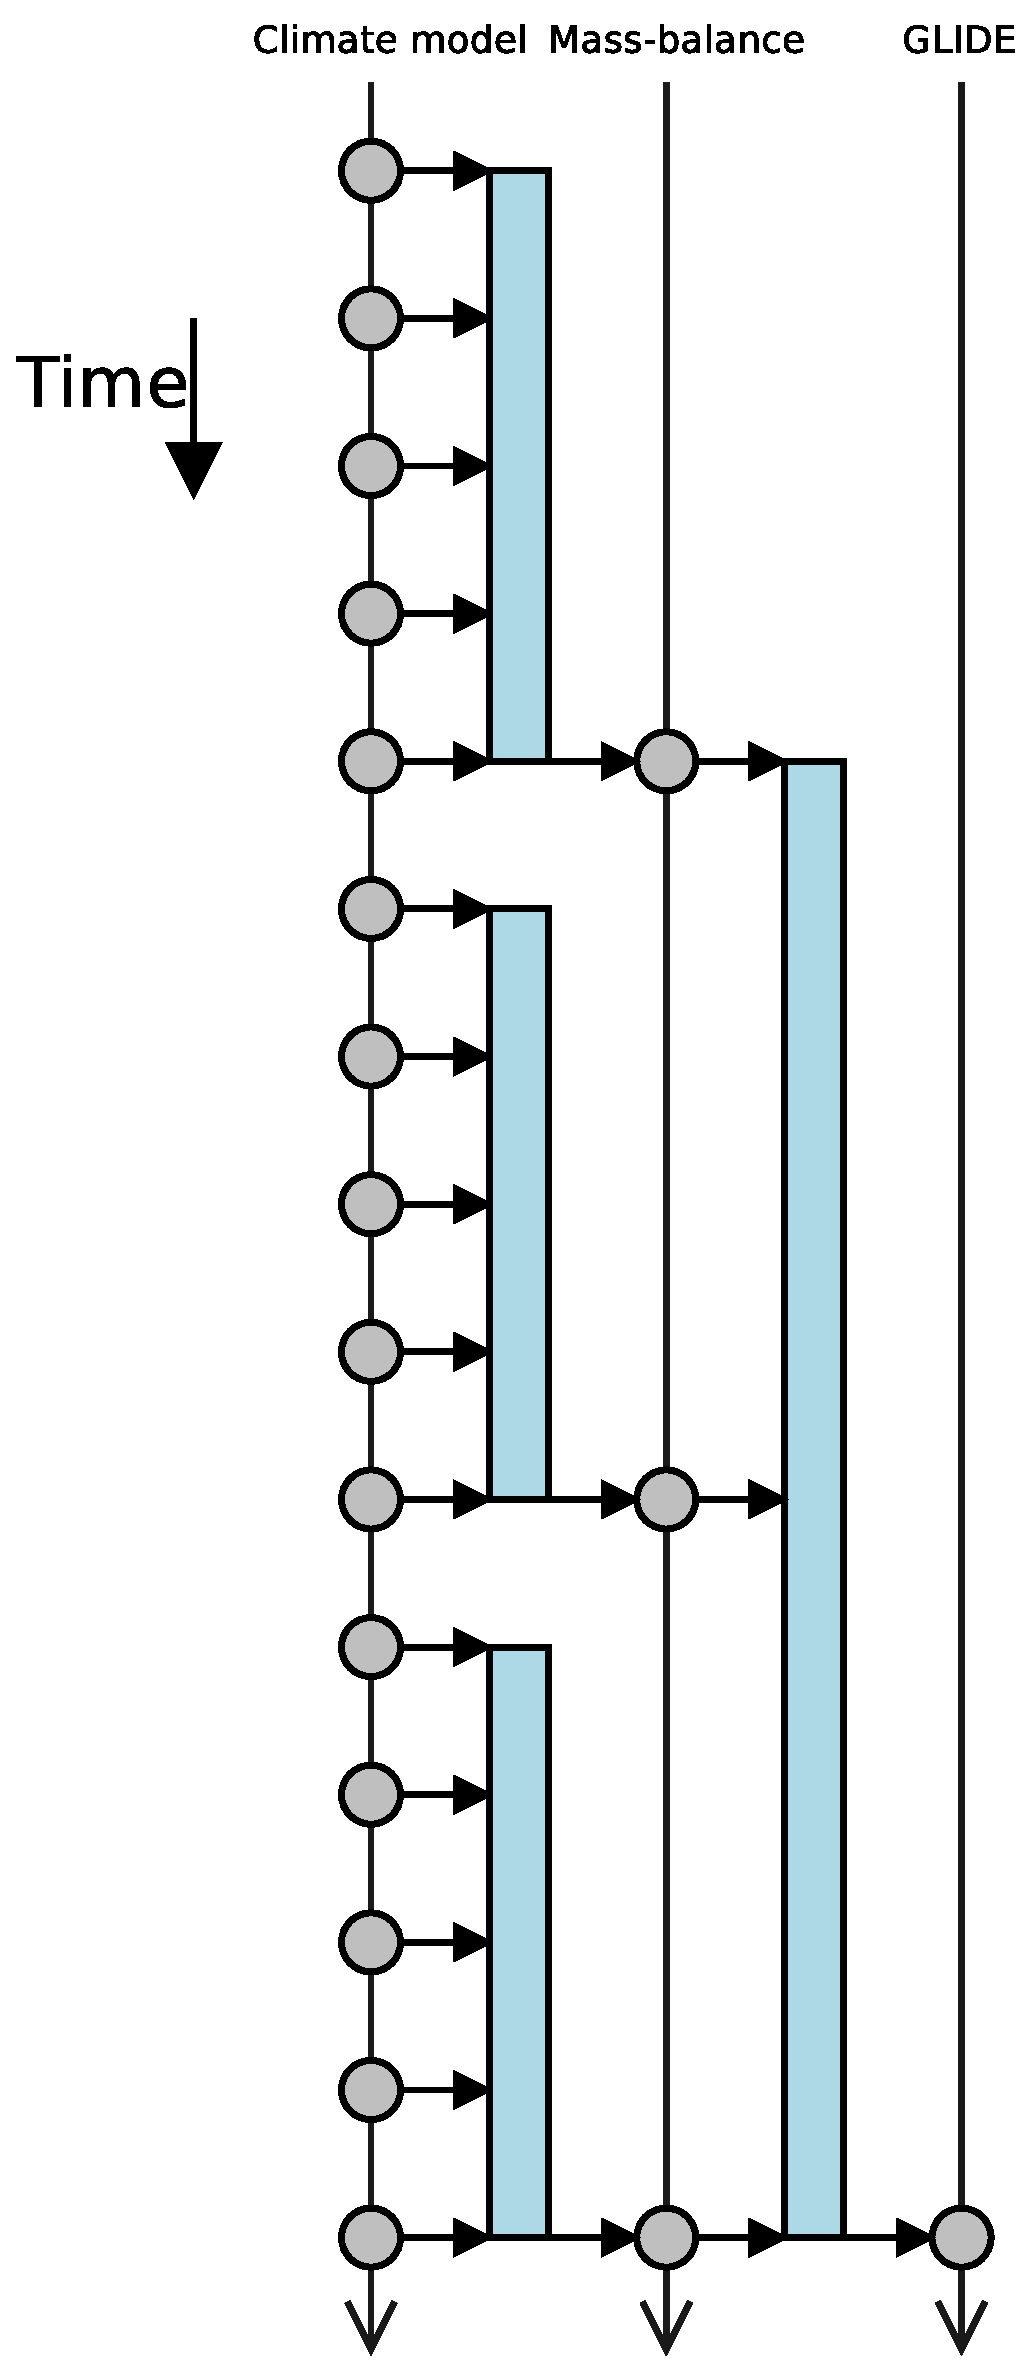
\includegraphics[width=0.6\textwidth]{\dir/figs/glint_timesteps.eps}
%  \caption{Relationship between the timesteps in GLINT. The filled circles
%  represent timesteps, the rectangles represent averaging/accumulation, and the arrows,
%  flow of coupling fields. \textbf{DO WE STILL WANT THIS FIGURE? IS IT STILL ACCURATE?}}
%  \label{ug.fig.glint_timesteps}
%\end{figure}
%
\subsubsection{Prerequisites}
%
Glint users should bear the following in mind:
%
\begin{itemize}
\item Global input fields must be supplied on a latitude-longitude
  grid. The grid does not have to be uniform in latitude, meaning that
  Gaussian grids may be used. Irregular grids (e.g., icosahedral grids) are not
  currently supported. The boundaries of the grid boxes may be specified; if
  not, they are assumed to lie halfway between the grid points in lat-lon space.
\item In the global field arrays, latitude must be indexed from north to south.
  That is, the first row of the array is the northernmost one. (Some
  flexibility might be introduced here in the future.)
\item The global grid must not have grid points at either of the
  poles. This restriction is not expected to be permanent, and in the meantime
  can probably be overcome by moving the location of the polar points to be
  fractionally short of the pole (e.g. at 89.9$^{\circ}$ and -89.9$^{\circ}$).
\end{itemize}
%
\subsubsection{Initializing and calling}
\label{ug.call_glint}

The easiest way to learn how Glint is used is by way of an
example. Glint should be built automatically as part of CISM, and we assume
here that this has been done successfully.

Typically, Glint will be called from the main program body of a
climate model. (In CESM, Glint subroutines are called from a wrapper layer
called \bf{glc}}.)  To make this possible, the compiler needs to be told to use the
Glint code, with ``use'' statements like the following:
%
\begin{verbatim}
  use glint_main
\end{verbatim}
%
The next task is to declare a variable of type \texttt{glint\_params}, which
holds everything relating to the model, including any number of ice-sheet
instances:
%
\begin{verbatim}
  type(glint_params) :: ice_sheet
\end{verbatim}
%
Before the ice-sheet model may be called from the climate model, it must be
initialized. This can be done with the following subroutine call\footnote
{The spelling of some subroutine names reflects the British origins
of the code.}:
%
\begin{verbatim}
  call initialise_glint(ice_sheet,lats,lons,time_step,paramfile)
\end{verbatim}
%
These are the required arguments; many optional arguments are also possible.
The required arguments are defined as follows:
%
\begin{itemize}
\item \texttt{ice\_sheet} is the variable of type \texttt{glint\_params}
 defined above;
\item \texttt{lats} and \texttt{lons} are one-dimensional arrays giving the
  locations of the global grid-points in latitude and longitude, respectively;
\item \texttt{time\_step} is the intended interval between calls to Glint, in
hours. This is known as the \emph{forcing timestep}. 
\item \texttt{paramfile} is the name of the Glint configuration file.
The contents of this file are discussed below. 
\end{itemize}

If Glint is to be forced with an externally computed surface mass balance
(rather than the fields that would drive a PDD scheme), the climate model
should instead call the subroutine \texttt{initialise\_glint\_gcm},
which has the same required arguments but a different set of optional arguments.

After Glint is initialised, it may be called as part of the main climate
model time-step loop:
%
\begin{verbatim}
    call glint(ice_sheet,time,temp,precip,orog)
\end{verbatim} 
%
where
%
\begin{itemize}
\item \texttt{ice\_sheet} is the variable of type \texttt{glint\_params} defined above;
\item \texttt{time} is the current model time, in hours;
\item \texttt{temp} is the daily mean $2\,\mathrm{m}$ global air temperature field, in
  $^{\circ}\mathrm{C}$;
\item \texttt{precip} is the global daily accumulated precipitation field,
  in $\mathrm{mm}$ (water equivalent, making no distinction
  between rain, snow, etc.);
\item \texttt{orog} is the global orography field, in $\mathrm{m}$.
\end{itemize}
Many optional arguments may also be specified.

The latter three compulsory fields are needed to drive a PDD scheme.
Glint includes two such schemes.  One of these calculates the mass-balance for the
whole year (the \emph{annual PDD scheme}), while the other calculates on a
daily basis (the \emph{daily PDD scheme}). The annual scheme incorporates a
stochastic temperature variation to account for diurnal and other variations,
which means that if this scheme is used, Glint should be called such
that short-term variations have been removed.  In practice, this means calling 
Glint on a monthly basis, with monthly mean temperatures. 
For the daily scheme, no such restriction exists,
and the scheme should be called at least every 6 hours.

If the SMB is computed externally by a climate model, the call to Glint would resemble this one:
\begin{verbatim}
    call glint_gcm(ice_sheet,time,qsmb,tsrf,topo)
\end{verbatim} 
%
where the last three arguments (all compulsory) are defined as follows:
%
\begin{itemize}
\item \texttt{qsmb} is the surface mass balance in kg m$^{-2}$ s$^{-1}$;
\item \texttt{tsrf} is the surface ground temperature in $^{\circ} C$, used as an upper 
thermal boundary condition for the ice sheet; and
\item \texttt{topo} is the surface elevation in m.
\end{itemize}
These fields contain two horizontal dimensions, along with a third dimension
for elevation class.  CESM typically computes these quantities in 10 elevation classes
per glaciated grid cell in the climate model.

Among the optional arguments are the following output fields (returned by Glint to the climate model):
\begin{itemize}
\item \texttt{gfrac} is the fractional grid cell area covered by ice;
\item \texttt{gtopo} is the mean surface elevation in m;
\item \texttt{ghflx} is the upwelling heat flux at the ice sheet surface, in W m$^2$;
\item \texttt{grofi} is the solid runoff flux (i.e., the calving flux) in kg m$^{-2}$ s$^{-1}$;
\item \texttt{grofl} is the liquid runoff flux in kg m$^{-2}$ s$^{-1}$.
This includes basal and possibly internal melting, but not surface melting
(which has already been computed by the climate model).
\end{itemize}
%
These fields are required by CESM to update its land-surface types and topography and to conserve heat
and water when CISM is coupled interactively to the climate model.  
The first three fields are computed for each elevation class in each climate model grid cell,
and the two runoff fluxes are averaged over each grid cell.
The initial ``g'' denotes that these fields have been upscaled to the global climate grid.
%
\subsubsection{Finishing off}
%
After the desired number of time steps have been run, Glint may have some
tidying up to do. To do this, the subroutine \texttt{end\_glint}
must be called:
%
\begin{verbatim}
  call end_glint(ice_sheet)
\end{verbatim}
%
%WHL - Commented out this subsubsection, since the API material has been commented out in the appendices.
%\subsubsection{API}
%
%A detailed description of the Glint API may be found in the appendices.
%
\subsubsection{Configuration}
%
Glint uses the same configuration file format as the rest of CISM. If
there is only one ice sheet instance, all the configuration data for
Glint and Glide (or Glissade) can reside in the same file.  If two or more instances are
used, a top-level file specifies the number of model instances and the name of
a configuration file for each one. Configuration sections specific to
Glint are as follows:
%
\begin{center}
  \tablefirsthead{%
    \hline
  }
  \tablehead{%
    \hline
    \multicolumn{2}{|p{0.98\textwidth}|}{\emph{\small continued from previous page}}\\
    \hline
  }
  \tabletail{%
    \hline
    \multicolumn{2}{|r|}{\emph{\small continued on next page}}\\
    \hline}
  \tablelasttail{\hline}
  \begin{supertabular}{|l|p{11cm}|}
%%%% 
    \hline
    \multicolumn{2}{|l|}{\texttt{[Glint]}}\\
    \hline
    \multicolumn{2}{|p{0.98\textwidth}|}{Section specifying number of instances.}\\
    \hline
    \texttt{n\_instance} & (integer) Number of instances (default=1)\\
    \hline
%%%% 
    \hline
    \multicolumn{2}{|l|}{\texttt{[Glint instance]}}\\
    \hline
    \multicolumn{2}{|p{0.98\textwidth}|}{Specifies the name of an
    instance-specific configuration file. Unnecessary if we only have one
    instance whose configuration data is in the main config file.}\\
    \hline
    \texttt{name} & Name of instance-specific config file (required).\\
    \hline
%%%% 
    \hline
    \multicolumn{2}{|l|}{\texttt{[Glint climate]}}\\
    \hline
    \multicolumn{2}{|p{0.98\textwidth}|}{Glint climate configuration}\\
    \hline
    \texttt{evolve\_ice} & {\raggedright
      specify whether or not the ice sheet evolves in time: \\
      \begin{tabular}{lp{10cm}}
        0 &  Do not evolve ice sheet (hold fixed in time). This setting is appropriate if we want to
        analyze the SMB downscaled to the observed ice sheet geometry, without the complexity of evolution.\\
        {\bf 1} & Allow the ice sheet to evolve \\
      \end{tabular}}\\
    \texttt{precip\_mode} & {\raggedright
      Method of precipitation downscaling: \\
      \begin{tabular}{lp{10cm}}
        {\bf 1} & Use large-scale precipitation rate\\
        2 & Use parameterization of \emph{Roe and Lindzen}\\
      \end{tabular}}\\
    \texttt{acab\_mode} & {\raggedright
      Mass-balance model to use:\\
      \begin{tabular}{lp{10cm}}
        0 & The surface mass balance is computed externally (e.g., by a climate model)\\
        {\bf 1} & Annual PDD mass-balance model (Section~\ref{ug.mbal.pdd_scheme})\\
        2 & Annual accumulation only\\
        3 & Hourly energy-balance model (NOTE: not supported) \\
        4 & Daily PDD mass-balance model (Section \ref{ug.mbal.daily_pdd_scheme})\\
      \end{tabular}}\\
    \texttt{ice\_albedo} & Albedo of ice---may be used for coupling to climate
    model (default=0.4) \\
    \texttt{lapse\_rate} & Atmospheric temperature lapse-rate, used to correct
    the atmospheric temperature onto the ice model orography. This should be
    \emph{positive} for temperature falling with height
    ($\mathrm{K}\,\mathrm{km}^{-1}$) (default=8.0) \\
    %%%%%%%%%%%%%%
    \texttt{data\_lapse\_rate} & Atmospheric temperature vertical lapse rate,
    to be used in the calculation of temperature at
    sea level. The variable \texttt{lapse\_rate} is then used to adjust the
    temperature to the surface of the local ice sheet topography. If
    \texttt{data\_lapse\_rate} is not set, it is set to the value of
    \texttt{lapse\_rate} by default. \\
    %%%%%%%%%%%%%%
    \texttt{ice\_tstep\_multiply} & Ice time-step multiplier: allows
    asynchronous climate-ice coupling. See below for full explanation of Glint
    time-stepping. (default = 1) \\
    %%%%%%%%%%%%%%
    \texttt{mbal\_accum\_time} & Mass-balance accumulation time (in years,
    default is equal to mass-balance timestep).  See below for full explanation of Glint
    time-stepping. \\
    \hline
  \end{supertabular}
\end{center}

\subsubsection{Glint timestepping --- an explanation}

By default, the model accepts input on each forcing timestep (as specified in 
the call to \texttt{initialise\_glint}). Input fields are accumulated over the course 
of a mass-balance time-step, whereupon the mass-balance model is called. The 
output from the mass-balance model is accumulated over the course of an ice sheet
model time-step, and finally the ice sheet model (Glide or Glissade) is called.

This default behaviour can be altered, in two ways:
\begin{enumerate}
\item The number of ice sheet time steps executed for each accumulated 
mass-balance field may be increased---thus accelerating the ice sheet relative 
to the forcing. To do this, set \texttt{ice\_tstep\_multiply} in the \texttt{[Glint climate]} 
config section; this must be an integer. This acceleration is possible only if the 
mass balance is accumulated over an integer number of years.
\item The mass-balance accumulation period can be altered by setting  
\texttt{mbal\_accum\_time} in the \texttt{[Glint climate]} config section; this is a 
floating-point value in years.
\end{enumerate}
%
The interaction of these two parameters is fairly complex, and permits
sophisticated control of how the ice sheet model is forced. 
Various checks are made at run-time to make sure that sensible values are selected. Most 
importantly, all relevant time-steps must divide into one another 
appropriately. The model will (or should) stop if an un-sensible combination 
of values is detected.

\subsubsection{Glint timestepping --- further examples}

To aid understanding of the time-stepping controls, here are some examples. First, suppose we have these time-step values:

\vspace{0.5cm}
\begin{tabular}{ll}
forcing time-step: & 6 hours \\
mass-balance time-step: & 1 day \\
ice time-step: & 0.5 year
\end{tabular}
\vspace{0.5cm}
%
By default, the model will accumulate 6 months of mass-balance 
calculations, and force the ice sheet model based on the 6-month average. This might not be 
desirable, so you could set:
%
\begin{verbatim}
    mbal_accum_time = 1.0
\end{verbatim}
%
This would make Glint accumulate 1 year of mass-balance output before 
forcing the ice sheet (at which point it would execute \emph{two} ice sheet 
time-steps of 0.5 years each).

Having done that, you could accelerate the ice model by a factor of ten, by 
setting

\begin{verbatim}
    ice_tstep_multiply = 10
\end{verbatim}
%
In this scenario, 20 ice sheet time-steps of 0.5 years each would be done 
after each 12-month accumulation of mass-balance data.

For the second example, we consider the contrasting situation where we do not want to calculate a 
mass balance on all the available data (perhaps to save time). Consider 
these time-step values:

\vspace{0.5cm}
\begin{tabular}{ll}
forcing time-step:   &   6 hours \\
mass-balance time-step: & 1 day \\
ice time-step:       &   10 years\\
\end{tabular}
\vspace{0.5cm}
%
(Clearly this is a numerically stable and/or low-resolution ice sheet).
To avoid running the daily PDD scheme c.3600 times (depending on the value of 
\texttt{days\_in\_year}), we can choose to use only the first two years of data:

\begin{verbatim}
    mbal_accum_time = 2.0
\end{verbatim}
%
Glint accumulates the mass balance for 2 years, then waits for 8 years (ignoring incoming 
data during this time) before calling the ice sheet. Ice sheet 
acceleration may be enabled with \texttt{ice\_tstep\_multiply} as before.

%________________________________________________
%________________________________________________
%
%   Glint example described here
%________________________________________________
%________________________________________________


\section{Glint: Using glint-example}
\label{ug.use_glint}
To run CISM using the Glint climate driver, go to directory \texttt{tests/glint\_example} 
and see the \texttt{README.glint\_example} file.
This file gives directions for downloading a tar file,
\texttt{glint-example.1.0.0.tar.gz}, that contains three data files
used to force Glint:
%
\begin{itemize}
\item \texttt{ncep-doe\_6h\_climate.64x32.nc} consists of 6-hourly precipitation and
surface temperature data on a coarse global grid;
\item \texttt{orog.igcmgrid.64x32.nc} consists of surface elevation data on a global grid
(these data are used to downscale temperature as a function of elevation); and
\item \texttt{gland20.input.nc} includes thickness and topography data for the Greenland 
ice sheet on a 20-km mesh.
\end{itemize}
%
These files should be placed in directory \texttt{tests/glint\_example}. 
This directory already includes the following config files:
\begin{itemize}
\item \texttt{greenland\_20km.config.pdd} and \texttt{greenland\_20km.config.smb} are
ice sheet configuration files for PDD and SMB forcing, respectively;
\item \texttt{glint\_example.config.pdd} and \texttt{glint\_example.config.smb} are the
corresponding climate configuration files.
\end{itemize}

To apply the PDD scheme, type
\begin{verbatim}
cism_driver greenland_20km.config.pdd glint-example.config.pdd
\end{verbatim}
%
and to apply the SMB scheme, type
\begin{verbatim}
cism_driver greenland_20km.config.pdd glint-example.config.pdd
\end{verbatim}
%
The 6-hourly temperature and precipitation data 
are tailored for a PDD scheme.  The same data, however, can also supply a crude
surface mass balance and surface temperature in multiple elevation classes, imitating
the forcing from a climate model such as CESM.  (Accumulation is set equal to precipitation,
and ablation is assumed to be linearly related to the downscaled temperature.
This scheme is convenient for testing but obviously is not appropriate for science.)
By default, two files are output at a specified frequency: a history file
containing variables of interest (e.g., thickness, velocity, and SMB) is output every 10 years,
and a ``hot'' file containing the variables required for exact restart is output every 1000 years.
 
%________________________________________________
%________________________________________________
%
%   Surface Mass Balance and PDD schemes described here
%________________________________________________
%________________________________________________


\section{Supplied mass-balance schemes}

%** We don't use these for anything, and I don't know if any one of us knows about them in any detail. Have we tested them at all recently? If we aren't familiar with them perhaps we should not support them? **
%WHL - See the warning I added two paragraphs below.

Users are free to supply their own mass-balance model for use
with Glide. However, Glint includes two positive-degree-day models
for mass balance, one annual and one daily.
This section describes how to configure and call these models.

NOTE: CISM2 development has focused on CESM-style coupling where the SMB
is computed externally.  The two PDD schemes (and the following description)
are identical to those in the original Glimmer code, but the schemes 
have not been extensively tested. Users should proceed with caution.

\subsection{Annual PDD scheme}
\label{ug.mbal.pdd_scheme}
The annual PDD scheme is contained in the f90 module \texttt{glimmer\_pdd},
and the model parameters are contained in the derived type
\texttt{glimmer\_pdd\_params}. Configuration data is contained in a standard
CISM config file, which needs to be read before initializing the
mass-balance model. The model is initialized by calling the subroutine
\texttt{glimmer\_pdd\_init}, and the mass-balance may be calculated annually
by calling \texttt{glimmer\_pdd\_mbal}. 

\subsubsection{Example of use:}
\begin{verbatim}
  use glimmer_pdd
  use glimmer_config

  ...

  type(glimmer_pdd_params) :: pdd_scheme
  type(ConfigSection),pointer :: config

  ...

  call glimmer_pdd_init(pdd_scheme,config)

  ...

  call glimmer_pdd_mbal(pdd_scheme,artm,arng,prcp,ablt,acab)
\end{verbatim}
In the subroutine call to \texttt{glimmer\_pdd\_mbal}, apart from the
parameter variable \texttt{pdd\_scheme}, there are three input fields
(\texttt{artm}, \texttt{arng} and \texttt{prcp}), which are, respectively, the
annual mean air temperature, annual temperature half-range, and annual
accumulated precipitation fields. The final two arguments are output fields
--- annual ablation (\texttt{ablt}) and annual mass-balance
(\texttt{acab}). 
Temperatures are in degrees Celsius, and precipitation, ablation and mass-balance are measured in
m of water equivalent.
%

\subsubsection{Degree-day calculation}
%
The greater part of the information in the \texttt{glimmer\_pdd\_params}
derived type comprises a look-up table (the \emph{PDD table}). The model is
implemented this way for computational efficiency.

The table has two dimensions: mean annual air temperature ($T_a$)
(as the second index) and annual air temperature half range (i.e.,
from July's mean to the annual mean $\Delta T_a$) (as the first
index).  Following \emph{Huybrechts and others} [1991], daily air
temperatures ($T_a^\prime$) are assumed to follow a sinusoidal
cycle
\begin{equation}
    T_a^\prime = T_a + \Delta T_a \cos \left( \frac{2 \pi t}{A}
    \right) + \textbf{R}(0,\sigma)
\end{equation}
where $A$ is the period of a year and $R$ is a random fluctuation
drawn from a normal distribution with mean 0 $^\circ$C and
standard deviation $\sigma$ $^\circ$C. \emph{Huybrechts and
others} [1991] indicate that the number of positive degree days
(D, $^\circ$C days) for this temperature series can be evaluated
as
\begin{equation}\label{pdd}
    D = \frac{1}{\sigma \sqrt{2 \pi}}
    \int\limits_0^A
    \int\limits_0^{T_a^\prime+2.5\sigma}
    T_a \times \exp \left( \frac{-(T_a-T_a^\prime)^2}{2 \sigma^2} \right) dT
    dt
\end{equation}
where $t$ is time.  The table is completed by evaluating this integral using a
public-domain algorithm (Romberg integration) by {\it Bauer} [1961]. The
inner and outer integrals are coded as two subroutines
(\texttt{inner\_integral} and \texttt{pdd\_integrand}), which call the Romburg
integration recursively.

The main parameter needed is the assumed standard deviation of
daily air temperatures, which can be set in the configuration file (the
default is 5 $^\circ $C). 

The positive-degree days are then looked up in the table (as a function of
$T_a$ and $\Delta T_a$). We take care to check that this look up is in done
within the bounds of the table.  The final value of $P$ is determined using
bilinear interpolation given the four nearest entries in the table to the
actual values of $T_a$ and $\Delta T_a$.

The remainder of the loop completes the calculation of the
ablation and accumulation given this value for $P$.
%
\subsubsection{Mass balance calculation} 
%
We use the following symbols: $a$ is total annual ablation; $a_s$
is potential snow ablation; $b_0$ is the capacity of the snowpack
to hold meltwater by refreezing; the total number of positive
degree days ($D$); degree-day factors for snow and ice ($f_s$ and
$f_i$); and the fraction of snowfall that can be held in the
snowpack as refrozen meltwater ($W_{\textrm{max}}$). The
degree-day factors have been converted from ice to water
equivalents using the ratio of densities.

First, determine the depth of superimposed ice ($b_0$) that would have to
be formed before runoff (mass loss) occurs as a constant fraction
($W_{\textrm{max}}$) of precipitation ($P$):
\begin{equation}
    b_0=W_{\textrm{max}} P.
\end{equation}
Now determine the amount of snow melt by applying a constant
degree-day factor for snow to the number of positive degree-days:
\begin{equation}
    a_s=f_s D.
\end{equation}
We now compare the potential amount of snow ablation with the
ability of the snow layer to absorb the melt.  Three cases are
possible. First, all snow melt is held within the snowpack and no
runoff occurs ($a=0$).  Second, the ability of the snowpack to
hold meltwater is exceeded but the potential snow ablation is
still less than the total amount of precipitation so that
$a=a_s-b_0$. Finally, the potential snow melt is greater than the
precipitation (amount of snow available), so that ice melt ($a_i$)
has to be considered as well.  The total ablation is therefore the
sum of snow melt (total precipitation minus meltwater held in
refreezing) and ice melt (from the total number of degree-days,
deduct the number of degree-days needed to melt all snowfall and convert
to ice melt):
\begin{equation}
    a=a_s + a_i = P - b_0 + f_i \left( D-\frac{P}{f_s} \right).
\end{equation}
We now have a total annual ablation, and can find total net mass
balance as the difference between the annual precipitation
and the annual ablation.

This methodology is fairly standard and stems from a
series of Greenland papers by Huybrechts, Letreguilly and Reeh in
the early 1990s.
%
%
%
\subsubsection{Configuration}
The annual PDD scheme is configured using a single section in the
configuration file:
\begin{center}
  \tablefirsthead{%
    \hline
  }
  \tablehead{%
    \hline
    \multicolumn{2}{|p{0.98\textwidth}|}{\emph{\small continued from previous page}}\\
    \hline
  }
  \tabletail{%
    \hline
    \multicolumn{2}{|r|}{\emph{\small continued on next page}}\\
    \hline}
  \tablelasttail{\hline}
  \begin{supertabular}{|l|p{11cm}|}
%%%% 
    \hline
    \multicolumn{2}{|l|}{\texttt{[GLIMMER annual pdd]}}\\
    \hline
    \multicolumn{2}{|p{0.98\textwidth}|}{Specifies parameters for the PDD
    table and mass-balance calculation}\\
    \hline
    \texttt{dx} & Table spacing in the $x$-direction ($^{\circ}$C) (default=1.0)\\
    \texttt{dy} & Table spacing in the $y$-direction ($^{\circ}$C) (default=1.0)\\
    \texttt{ix} & Lower bound of $x$-axis ($^{\circ}$C) (default=0.0)\\
    \texttt{iy} & Lower bound of $y$-axis ($^{\circ}$C) (default=-50.0)\\
    \texttt{nx} & Number of values in x-direction (default=31)\\
    \texttt{ny} & Number of values in x-direction (default=71)\\
    \texttt{wmax} & Fraction of melted snow that refreezes (default=0.6) \\
    \texttt{pddfac\_ice} & PDD factor for ice (m day$^{-1}\,^{\circ}$C$^{-1}$)
    (default=0.008)\\
    \texttt{pddfac\_snow} & PDD factor for snow (m day$^{-1}\,^{\circ}$C$^{-1}$) (default=0.003)\\
  \end{supertabular}
\end{center}
\subsubsection{References}

\noindent Bauer (1961) \emph{Comm. ACM} \textbf{4}, 255.

\noindent Huybrechts, Letreguilly and Reeh (1991) \emph{Palaeogeography,
Palaeoclimatology, Palaeoecology (Global and Planetary Change)}
\textbf{89}, 399-412.

\noindent Letreguilly, Reeh and  Huybrechts (1991) \emph{Palaeogeography,
Palaeoclimatology, Palaeoecology (Global and Planetary Change)}
\textbf{90}, 385-394.

\noindent Letreguilly, Huybrechts  and  Reeh (1991) \emph{Journal of
Glaciology} \textbf{37}, 149-157.
%
%%%%%%%%%%%%%%%%%%%%%%%%%%%%%%%%%%%%%%%%%%%%%%%%%%%%%%%%%%%%%%%%%%%%%%%%%%%%%
% Daily PDD scheme
%%%%%%%%%%%%%%%%%%%%%%%%%%%%%%%%%%%%%%%%%%%%%%%%%%%%%%%%%%%%%%%%%%%%%%%%%%%%%
%
\subsection{Daily PDD scheme}
\label{ug.mbal.daily_pdd_scheme}
The other PDD scheme is a daily scheme. This is simpler than the annual scheme in that it does not incorporate any stochastic variations. The mass balance is calculated on a daily basis, given the daily mean temperature and half-range, and assuming a sinusoidal diurnal cycle. Consequently, the firn model is more sophisticated than with the annual scheme, and includes a snow-densification parameterization.
%
\subsubsection{Configuration}
The daily PDD scheme is configured using a single section in the configuration file:
\begin{center}
  \tablefirsthead{%
    \hline
  }
  \tablehead{%
    \hline
    \multicolumn{2}{|p{0.98\textwidth}|}{\emph{\small continued from previous page}}\\
    \hline
  }
  \tabletail{%
    \hline
    \multicolumn{2}{|r|}{\emph{\small continued on next page}}\\
    \hline}
  \tablelasttail{\hline}
  \begin{supertabular}{|l|p{11cm}|}
%%%% 
    \hline
    \multicolumn{2}{|l|}{\texttt{[GLIMMER daily pdd]}}\\
    \hline
    \multicolumn{2}{|p{0.98\textwidth}|}{Specifies parameters for the PDD
    table and mass-balance calculation}\\
    \hline
    \texttt{wmax} & Fraction of melted snow that refreezes (default=0.6) \\
    \texttt{pddfac\_ice} & PDD factor for ice (m day$^{-1}\,^{\circ}$C$^{-1}$)
    (default=0.008)\\
    \texttt{pddfac\_snow} & PDD factor for snow (m day$^{-1}\,^{\circ}$C$^{-1}$) (default=0.003)\\
    \texttt{rain\_threshold} & Temperature above which precipitation is held to be rain ($^{\circ}$C) (default=1.0)\\
    \texttt{whichrain} & {\raggedright
      Which method to use to partition precipitation into rain and snow:\\
      \begin{tabular}{lp{7cm}}
        {\bf 1} & Use sinusoidal diurnal temperature variation \\
        2 & Use mean temperature only\\
      \end{tabular}}\\
    \texttt{tau0} & Snow densification timescale (s) (default=10 years)\\
    \texttt{constC} & Snow density profile factor C (m$^{-1}$) (default=0.0165)\\
    \texttt{firnbound} & Ice-firn boundary as fraction of density of ice (default=0.872)\\
    \texttt{snowdensity} & Density of fresh snow ($\mathrm{kg}\,\mathrm{m}^{-3}$) (default=300.0)\\
  \end{supertabular}
\end{center}


